\DiaryEntry{Interesting Integrals (9) and the Harmonic Addition Theorem}{2019-09-17}{Integrals}

We consider the integral

\bee
I = \int_0^1 \frac{\ln(x+1)}{x^2 + 1} dx
\eee

We use the substitution $x = \tan u$ from which we have $\frac{dx}{du}=1 + \tan^2 x$ and our integral becomes

\bee
I = \int_{u=0}^{\pi/4} \frac{\ln(\tan^2 u +1)}{\tan^2 u +1} (1 + \tan^2 u) du = \int \ln \frac{\sin u + \cos u}{cos u} du = \int \ln (\sin u + \cos u) - \ln (\cos u) du
\eee

The harmonic addition theorem allows to express the sum of sine and cosine as follows

\bee
a \sin x + b \cos x = A \cos(x + \alpha) = A \left( \cos x \cos \alpha - \sin x \sin \alpha \right)
\eee

We now compare coefficients of $\cos x $ and $\sin x$ and obtain the following two equations

\begin{align*}
  a &= -A \sin \alpha \\
  b &= A \cos \alpha
\end{align*}

We first consider $a^2 + b^2 = A^2 \sin^2 \alpha + A^2 \cos^2 \alpha = A^2$ and then $\frac{a}{b} = -\tan \alpha$. So we have

\bee
A^2 = a^2 + b^2, \quad \frac{a}{b} = -\tan \alpha \qed
\eee

This allows us to rewrite $\sin u + \cos u$ from our above integral as

\bee
\sin u + \cos u = \sqrt{2} \cos \left(u - \frac{\pi}{4} \right)
\eee

Inserting back into the integral yields

\bee
I = \int_0^{\pi/4} \ln \left(\sqrt{2} \cos \left(u - \frac{\pi}{4} \right)\right) - \ln(\cos u) du = \int_0^{\pi/4} \ln (\sqrt{2}) + \ln \left(\cos \left(u - \frac{\pi}{4} \right)\right) - \ln(\cos u) du
\eee

This looks (still) intimidating, but a plot (see Figure below) shows that the areas below $\cos u$ and $\cos \left(u - \frac{\pi}{4} \right)$ are the same. Therefore also the log is the same and the last two expression int he integral cancel.

\begin{figure}[hbt!]
\centering
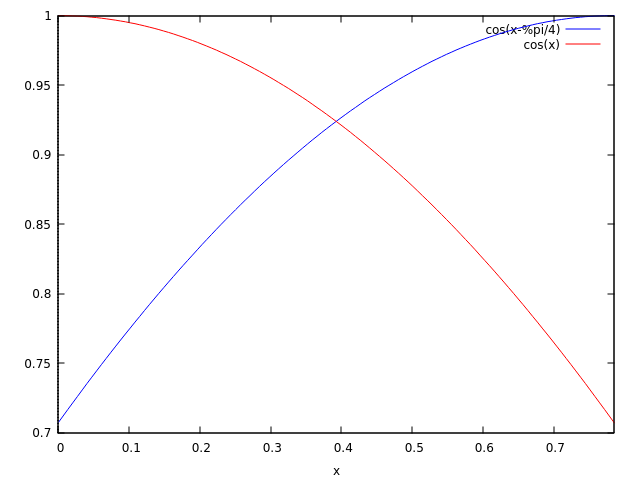
\includegraphics[scale=0.75]{images/interesting_integrals_09_1.png}
\end{figure}

So we arrive at

\bee
I = \frac{\pi}{4} \ln(\sqrt{2}) = \frac{\pi}{8} \ln 2 \approx 0.272 \qed
\eee

For the fun of it, we plot the integrand as well; see Figure below. Maxima seems to be able to solve the indefinite integral, but I don't get a meaningful result for $\int_0^\infty$; not sure if this converges.

\begin{figure}[hbt!]
\centering
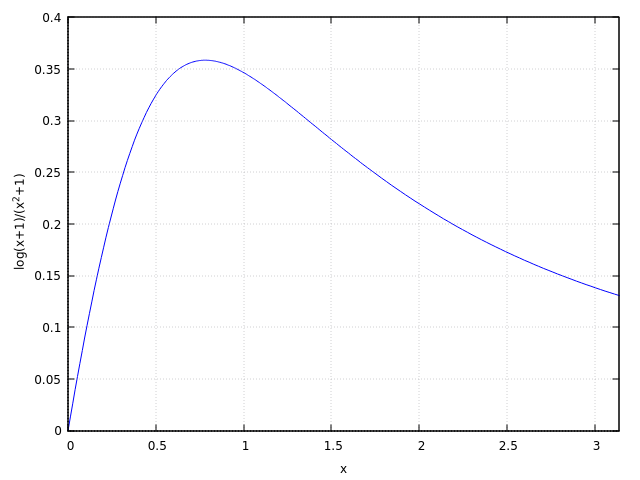
\includegraphics[scale=0.75]{images/interesting_integrals_09_2.png}
\end{figure}



%%% Local Variables:
%%% mode: latex
%%% TeX-master: "journal"
%%% End:
